%% PNAStwoS.tex
%% Sample file to use for PNAS articles prepared in LaTeX
%% For two column PNAS articles
%% Version1: Apr 15, 2008
%% Version2: Oct 04, 2013

%% BASIC CLASS FILE
\documentclass{pnastwo}

%% ADDITIONAL OPTIONAL STYLE FILES Font specification

%\usepackage{pnastwoF}
%\usepackage{cite}
\usepackage[numbers,round,compress]{natbib}
\bibpunct{(}{)}{,}{n}{,}{,}  % https://xianblog.wordpress.com/tag/natbib/ (allows natbib with PNAS)
\usepackage{lineno}
\setlength\linenumbersep{2pt}

%% OPTIONAL MACRO DEFINITIONS
\def\s{\sigma}
%%%%%%%%%%%%
%% For PNAS Only:
\url{www.pnas.org/cgi/doi/10.1073/pnas.0709640104}
\copyrightyear{2008}
\issuedate{Issue Date}
\volume{Volume}
\issuenumber{Issue Number}
%\setcounter{page}{2687} %Set page number here if desired
%%%%%%%%%%%%

\begin{document}

\title{Quantifying the impacts of bias in landcover data on global change analyses}

\author{Lyndon Estes\affil{1}{Princeton University, Princeton, NJ USA},
Peng Chen\affil{2}{Indiana University, Bloomington, IN USA},
Stephanie Debats\affil{1}{Princeton University, Princeton, NJ USA},
Tom Evans\affil{2}{Indiana University, Bloomington, IN USA},
Fanie Ferreira\affil{3}{GeoTerraImage, Pretoria, RSA},
Gabrielle Ragazzo\affil{1}{Princeton University, Princeton, NJ USA},
Justin Sheffield\affil{1}{Princeton University, Princeton, NJ USA}
\and
Kelly Caylor\affil{1}{Princeton University, Princeton, NJ USA}}

\contributor{Submitted to Proceedings of the National Academy of Sciences
of the United States of America}

%%%Newly updated.
%%% If significance statement need, then can use the below command otherwise just delete it.
%\significancetext{LDE developed the concept of the study, conducted the analysis, data interpretation and drafted the manuscript. \color{red}{To be completed}}

\maketitle

\begin{article}
\begin{abstract}
{Blah blah.}
\end{abstract}

\keywords{landcover | bias | remote sensing | agriculture | crop yield | harvested area | carbon | agent-based model | landscape}

\abbreviations{GTI, GeoTerraImage; SSA, sub-Saharan Africa}
\linenumbers

\dropcap{T}he nature and distribution of landcover is a fundamental determinant of many environmental and social processes that drive or are affected by global change \cite{lambin_modelling_1997}, such as agricultural production and food security \cite{lark_cropland_2015,wright_recent_2013, licker_mind_2010}, carbon cycling \cite{asner_high-resolution_2010,gaveau_major_2014}, biodiversity loss \cite{newbold_global_2015,luoto_predicting_2004}, or demographic changes \cite{linard_assessing_2010}. Landcover maps are therefore critical for understanding the nature and impact of such changes \cite{see_improved_2015}, and they need to be accurate at the finest scales at which the underlying processes operate. For example, agricultural productivity and nutrient loadings can vary greatly between neighboring fields, and field sizes are often $<$2 hectares in regions where smallholder farming still dominates \cite{jain_mapping_2013, debats_generalized_????}. To understand agriculturally driven processes, it is thus necessary to accurately delineate fields at their smallest grain size, and to do so at regional to global scales to have a consistent set of maps.   

Landcover data can only be developed with satellite imaging, but often the average size class of the cover type of interest is smaller than the sensor resolution, or spectrally indistinct from other neighboring covers, which propagates classification error \cite{see_improved_2015,lobell_use_2013,estes_diylandcover:_2015}. The result is that landcover datasets are generally inaccurate at finer scales and greatly differ between one another, particularly in those parts of the world undergoing the most rapid land use changes, where the aforementioned sources of bias tend to be most pronounced \cite{estes_projected_2013,fritz_comparison_2010,fritz_cropland_2011}.  

These errors are well-known \cite{fritz_comparison_2010, fritz_cropland_2011, see_improved_2015, fritz_mapping_2015,verburg_challenges_2011}, and there are a variety of efforts underway to improve landcover maps, particularly for agriculture \cite{fritz_geo-wiki:_2012,estes_diylandcover:_2015}. What is less known is the degree to which these errors bias measurements built upon the distributional and areal information in landcover. An impediment to this understanding is that the errors are hard to quantify because spatially extensive reference data are not available for most regions of the world--particularly over Africa and other developing regions. Errors assessment therefore typically rely on a small number of ground truth points or survey data aggregated to political boundaries. For this reason, we have a better understanding of the biases between landcover datasets or in relation to country-level statistics \cite{fritz_comparison_2010,fritz_cropland_2011,kaptue_tchuente_comparison_2011} than we do of how error changes over spatial gradients or as a function of aggregation scale. 

Being unable to fully quantify the errors in landcover maps of course makes it difficult, if not impossible, to quantify their impact on downstream analyses. There has been some work examining how such error influences climate simulations \cite{ge_impacts_2007}, agricultural land use patterns \cite{schmit_limitations_2006}, and carbon flux \cite{quaife_impact_2008} and human population estimates \cite{linard_assessing_2010}, but these either use simulated landcover errors \cite{ge_impacts_2007} or compare relevant differences in estimates between different satellite-derived landcover maps \cite{linard_assessing_2010, quaife_impact_2008}. The exception is \cite{schmit_limitations_2006}, who use a high quality, ground-collected reference map detailing farm land use parcels in central Belgium, but the number of sites and region were both fairly restricted, and the parcels were not spatially contiguous. 

There is thus an urgent need to more precisely quantify landcover map errors and how these vary over large regions, particularly for the regions where landcover is changing most rapidly yet is most poorly known.  We address this need in this study, using a unique, high accuracy agricultural landcover map for South Africa to quantify the errors in several latest generation landcover maps that are broadly used in global change studies.  We use this information to examine how i) landcover properties and related classification schemes influence error, ii) how these errors change with aggregation scale, with the specific goal of determining ``safe'' scales for making area-based calculations, and 3) how these errors propagate through several different forms of downstream analyses that broadly represent the global change research focus areas, including biogeochemical and land use change studies, food security assessments, land surface hydrology and climatology, and human geography.  

\vspace{-0.5 cm}
\section{Study area and landcover data}
Our study focused on South Africa, which comprises nearly 6\% of sub-Saharan Africa's (SSA) landmass, and has a large, diverse agricultural sector, ranging from large commercial operations to smallholder farms \cite{hardy_rainfed_2011,estes_using_2014}. This diversity suggests that the country's agricultural landcover spans the range of types that are found throughout the rest of SSA.  

The South African government commissioned a whole country cropland boundary map in order to stratifying the annual aerial crop type census used to calculate harvested area estimates \cite{fourie_better_2009}. The map was made by trained workers who visually interpreted high resolution satellite imagery and manually digitized field boundaries following a standardized mapping protocol. The resulting vectorized field maps, which were made in 2007 and updated in 2011, provide a unique, high accuracy reference dataset of both crop field distribution and size classes.  We converted the vector data into a rasterized estimated of cropland percentage at 1 km resolution (henceforth the ``reference map''), which was 97\% accurate in distinguishing cropped from non-cropped areas. 

We compared our reference percent cropland estimates to those created from four satellite-derived landcover datasets. We obtained South Africa's 30 m resolution National Landcover map (SA-LC) for 2009 \cite{sanbi_national_2009}, the 500 m resolution MODIS Landcover for 2011 \cite{land_processes_distributed_active_archive_center_lp_daac_modis_2011, friedl_modis_2010}, the 300 m resolution GlobCover 2009 \cite{arino_global_2012}, and the new 1 km Geo-wiki hybrid-fusion cropland map for Africa \cite{fritz_mapping_2015}. We chose these particular datasets because they are nearly contemporaneous with our reference data, and represent the major types of landcover products used by researchers: SA-LC typifies the higher resolution, Landsat-derived maps that are developed individually for many countries \cite{fry_completion_2009},  MODIS and GlobCover are widely used global-scale products \cite{gross_monitoring_2013,shackelford_conservation_2015}, while Geo-Wiki incorporates the first three datasets and is the current state of the art for agricultural landcover maps. We extracted the cropland classes from the first three datasets and converted these to 1 km resolution percent cropland estimates (hereafter simply the ``landcover maps''), resulting in 4 maps to compare to our reference cropland map (the ``reference map'').  

\vspace{-0.5 cm}
\section{Quantifying Error}
We used these maps to first quantify error in cropland area estimates. We calculated error as the difference between the reference and landcover maps at different scales of aggregation (1 to 100 km), in order to estimate bias and how it varies with scale. Next, we assessed how bias correlates with the amount of cropland cover in agricultural landscapes, to gain insight into how landscape patterns may affect error.    

We undertook five further analyses to investigate how map error can impact assessments founded on landcover maps. These include first-order analyses, in which values for a variable of interest are mapped to particular cover type(s), and second-order analyses, in which a process model draws on the cover types' values to calculate an output value. We created four datasets to represent second order analyses. The first was a series of maps of vegetated carbon stocks created following the methodology of Ruesch and Gibbs' \cite{ruesch_new_2008}. The second was constrained cropland percentage maps, which, following Ramankutty et al \cite{ramankutty_farming_2008} were adjusted so that their total cropland areas matched provincial-level reported cropland totals. Using these adjusted cropland percentage maps, we disaggregated district-reported maize harvested area and yields \cite[following][]{monfreda_farming_2008} . We then compared differences between total carbon stock estimates calculated from the reference map with those from the four cropland maps, and again examined how these differences changed as a function of aggregation scale.  We made the same comparisons for total maize harvested area, average yield, and total production. 

For the second-order analyses, we examined how cropland cover errors influence 25 km resolution monthly evapotranspiration estimates produced using the Variable Infiltration Capacity \cite{liang_simple_1994} land surface hydrology model. For this example, we used the cropland maps to adjust the seasonally varying, landcover-specific leaf area index (LAI) values that VIC uses to partition water vapor fluxes into their evaporative and transpirative components. In the second example, we examined how these errors can impact the parameterization of an agent-based food security model \cite{chen_dependency_2013}. Spatially-explicit, agent-based models are frequently employed in land change science, and require an initialization step to assign landscape resources to model agents  \cite[e.g.][]{manson_agent-based_2007,evans_multi-scale_2004,kelley_relative_2011}. In this case, we used the cropland maps to allocate farmland to agents representing individual households in political districts, with the model assigning each household its initial cropland holdings using a function that considers total district cropland and how much cropland is near the agent's location.  

\vspace{-0.5 cm}
\section{Results}
\subsection{Landcover bias}

We created the 1 km reference and landcover maps, removing all croplands marked as communal or smallholder farmland in the reference vector maps (individual fields were not mapped with the same precision), as horticulture, or plantation forestry (SI), and calculated the total cropland extent in the remaining area (1,081,000 km$^2$, or 90\% of South Africa).  The 2011 reference map showed a cropland area of 104,310 km$^2$, which the SA-LC and GeoWiki maps overestimated by 26 and 5.8\%, respectively, and GlobCover and MODIS underestimated by 21 and 26.1\%.  

We then aggregated each map to 5, 10, 25, 50, and 100 km resolutions, and subtracted the four landcover maps from the reference map at each scale of aggregation to asses the spatial patterns of bias (Fig. 1). 

\vspace{-0.25 cm}
\begin{figure}[ht]
\centerline{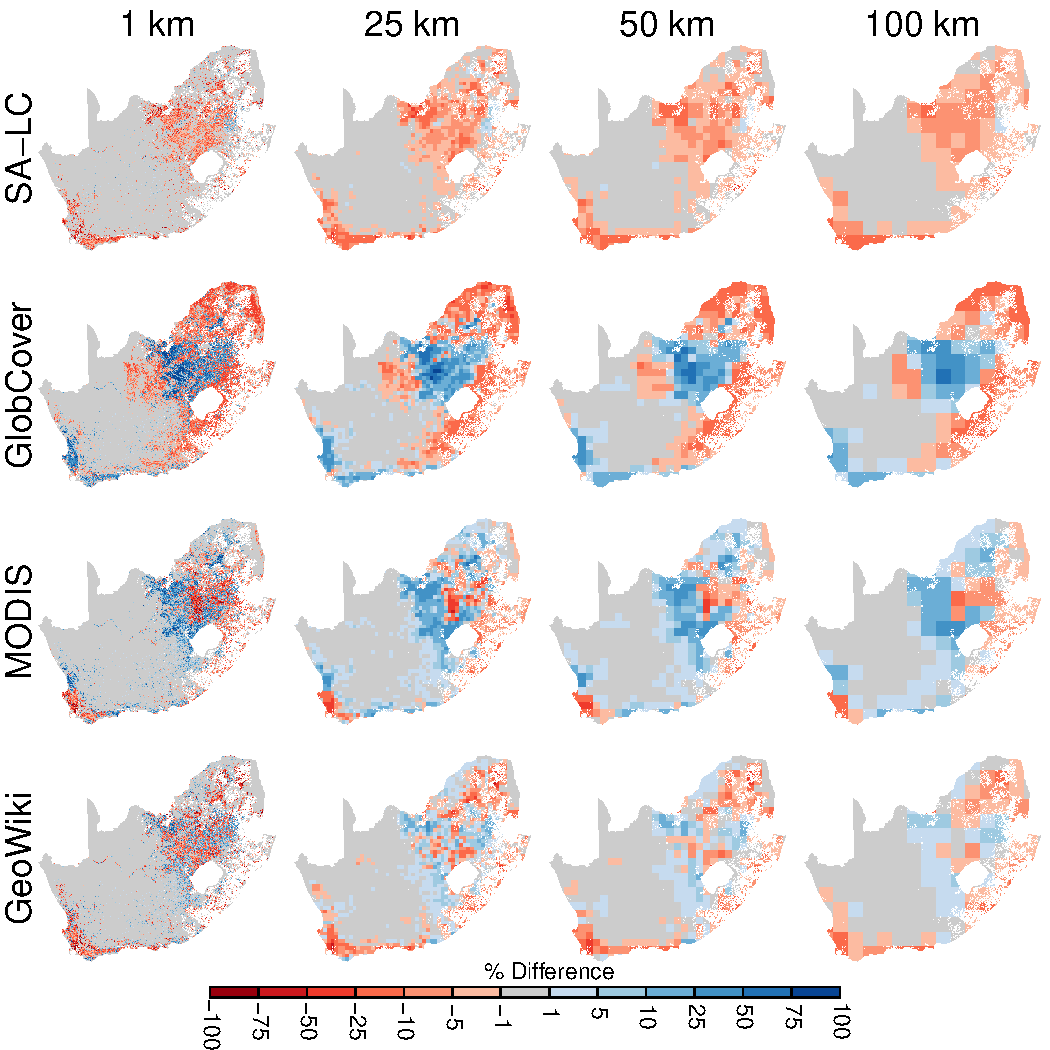
\includegraphics[width=.5\textwidth]{figures/bias_map.pdf}}
\caption{Differences in percent cropland estimates between the reference map and each of the four landcover maps. Rows indicate the landcover map being assessed (by subtraction from the reference map), while columns refer to resolution of aggregation. White indicates areas with no data where communal farmlands or plantation forests were removed.}\label{afoto}
\end{figure}

The most pronounced extreme biases are in the MODIS and GlobCover maps, with both underestimating cropland extent by 10-75\% in the center of the country (blue areas in Fig. 1, and the dominant production region), and overestimating along the eastern to northern margins (red areas in Fig. 1). The average biases for GlobCover and MODIS are 21\% and 34\% at 1 km, meaning that each map underestimates cropland by that amount at this resolution. MODIS mean bias drops to 8\% at 50 km of aggregation, whereas GlobCover bias is still 24\% at 100 km (SI Appendix, Fig. S1). 

The SA-LC map uniformly overestimates cropland throughout the country (Fig. 1), but the magnitude of mean bias is much lower at -8\% at 1 km to -6\% at 100 km  (Fig. S1). The GeoWiki map has a very heterogeneous pattern of bias, having a slight underestimation tendency (5\% mean bias) at 1 km, which changes to a smaller overestimation bias (-2 \%) at 100 km (Fig. S1).    

\subsection{The role of landscape characteristics in shaping bias}
To investigate the degree to which landscape features influence landcover map bias, we extract all pixels in agricultural areas ($>$0.5\% cropland) of the 1 km reference map using the the boundaries of 354 magisterial districts (South Africa's finest administrative unit, which average 3,445 km$^2$ in size; SI Appendix, Fig. S3), and averaged the values of these pixels within each district. These provided an estimate of the intensity of cropping within the farmed parts of the landscape (with districts defining the landscape scale), as well as the degree of mixing between cropland and other land covers. We then extracted the cropland map biases for the same locations, and calculated the mean absolute bias within each district. Absolute bias describes the magnitude of bias but not its direction, and is more informative about the likelihood of the map being biased at any given point in the landscape than actual bias, as positive and negative biases can cancel each other out within small areas. 

A generalized additive model fit to district-level absolute bias (log-transformed) shows that absolute bias peaks at 50\% cropland cover for all but the GlobCover map (which continued to increase with cropland cover), and is lowest when the landscape is dominated either by cropland or other cover types (Fig. 2). In other words, bias is highest when cropland cover is mixed evenly with other cover types. 

\vspace{-1 cm}
\begin{figure}[ht]
\centerline{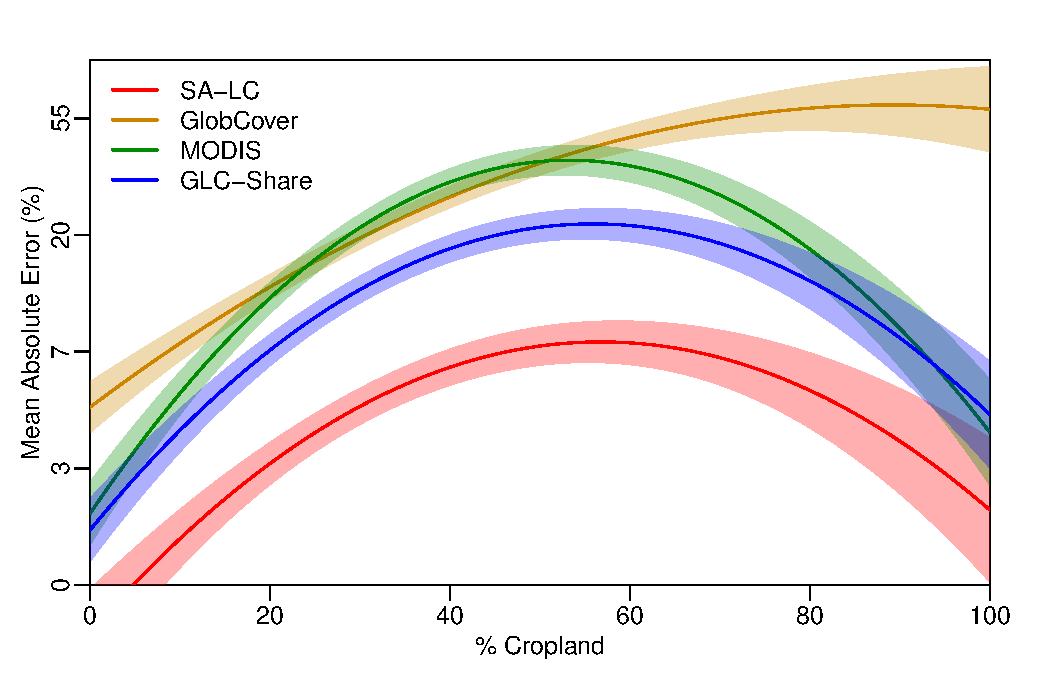
\includegraphics[width=.4\textwidth]{figures/biases_md_lnorm_gam_mu0.pdf}}
\caption{The relationship between the mean absolute bias in cropland maps and cropland cover within agricultural areas (reference map pixels having $>$0.5\% cropland), averaged within the boundaries of magisterial districts (n = 345), as fit with a generalized additive model. Prediction curves are color-coded to the different cropland maps, with the solid line indicating  predicted absolute bias, and the lighter shading the standard error of the coefficients. Models were also fit to the mean absolute biases across all four maps (black curve), and from all maps exlcuding GlobCover (grey surve).}
\label{afoto}
\end{figure}

\subsection{The impact of bias on calculating carbon stocks}
We used the data of \cite{ruesch_new_2008} to calculate carbon densities for African forests, shrublands, croplands, grasslands, and sparse habitats. We assigned the cropland carbon values to map cells in proportion to their cropland cover. For the non-cropland proportions, we assigned the carbon value from each of the other types, such that we created four  different carbon maps for each landcover map at each aggregation scale (Fig. S4), which allowed us to test how carbon estimates vary as a function of i) bias in the cropland estimates and ii) the characteristics of adjacent cover types. 

At the 1 km scale, the differences between country-wide total carbon stocks made using any of the cropland maps and the reference were within +/-3\%, regardless of which cover type was adjacent to cropland (Table S1), because differences between total stock estimates are diluted by the large area ($\sim$50-70\%) of the country having no cropland. Comparing the carbon stocks from each map's agricultural area reveals much greater differences (Table S1). SA-LC overestimates carbon stocks by just 2\% when the adjacent cover type is forest, and up to 15\% when it is spare cover. MODIS ranges from negligible overestimates in denser carbon classes (forest, secondary forest, and shrublands) to 8-13\% underestimates for the grassland and sparse classes. GeoWiki underestimates for all types, from $<$1\% for sparse cover to 8\% for forest. GlobCover shows the largest total carbon stock bias, with over-estimates ranging from for sparse lands to 162\% for forest. The magnitude of this bias is due to false positives--GlobCover identified cropland in nearly 50\% of pixels, compared to 30\% for the other three cropland maps. 

The spatial patterns of carbon bias (Fig. S4) are a reflection of the cropland biases (Fig. 1). Where cropland is underestimated and the surrounding cover type is of higher carbon density than cropland, carbon density is overestimated. For lower density (grassland and sparse vegetation), there may be slight underestimates.  These tendencies are reflected in the average of each map's spatial biases over agricultural areas (Fig. 3).  For example, MODIS and GlobCover overestimate carbon by $\sim$50\% on average at 1 km resolution when forest is the cropland-adjacent cover (stars in semi-transparent green and gold bars, Fig. 3; Table S2). When it is sparse vegetation (open circles in Fig. 3), MODIS underestimates by nearly 3\% at all scales, whereas maps that overestimate cropland (e.g. SA-LC, semi-transparent red) overestimate carbon density for this cover.  Overall, GeoWiki has the lowest average spatial biases, for all cover types and all resolutions. It's maximum bias is a 12\% overestimate at 1 km for forest cover, thereafter all biases are less than 10\%, and converge to +/-2\% above 1 km aggregation (Fig. 3, Table S2). All maps' biases are within +/-10\% bias after aggregation to 25 km.

\vspace{-0.9 cm}
\begin{figure}[ht]
\centerline{\includegraphics[width=.4\textwidth]{figures/carbon_veg_scale3.pdf}}
\caption{The average spatial biases in carbon density estimates based on cropland maps, expressed as a percent difference relative to the reference map. The values of actual bias (incorporating bias direction and magnitude) and absolute bias (magnitude only) are presented in semi-transparent and solid colors, respectively, with colors denoting the specific cropland map and symbols indicating which cover type was used to calculate cropland adjacent carbon density. The bar represents the mean biases calculated across each of the 5 cover types. Shrubland and grassland bias values are near zero and not shown for display clarity.}
\label{afoto}
\end{figure}

The patterns of mean absolute spatial bias (solid colored bars in Fig. 3) generally follow that of actual bias, but with somewhat higher magnitudes and a few notable differences. The most notable is that Geo-Wiki has fairly large absolute bias at 1 km, averaging 27\% across across cover types (line in solid blue bar, Fig. 3, Table S2), which is close to the 36-37\% for GlobCover and MODIS. SA-LC has the lowest absolute bias across scales, averaging (across cover types) from 14\% at 1 km to 3\% at 100 km. (Fig. 3, Table S2). The increase in Geo-Wiki's absolute spatial bias relative to SA-LC's can be attributed to the spatially heterogeneous nature of its cropland biases (Fig. 1) compared to the other three cropland maps.

\subsection{Bias in harvested areas, yield, and production estimates}

\begin{itemize}
  \item Used provincial boundaries to extract total cropland from reference data. Cropland totals used to adjust cropland fractions falling within those boundaries from each cropland map so cropland map totals equal the provincial-level total from the reference (SI). 
  \item Disaggregated magisterial district level maize yield and maize harvested area onto the adjusted cropland fractions, and onto the reference map.
  \item Calculated differences in spatial biases of yields and total production estimates at different scales of aggregation. 
  \item Yields aggregated to higher scale using two methods: 1) weighted mean aggregation, where harvested area fractions used to weight yields at each aggregation scale, technically more difficult; 2) mean of any harvested area contributing to aggregation, without weighting. Production aggregated by either calculating production at 1 km and then aggregating to each scale and differencing, or aggregating harvested fractions and type 2 yield, and calculating production at each level.
  \item Average bias normalized as a percentage of mean pixel-level yield or production calculated from the reference map.   
 \end{itemize}


\vspace{-1 cm}
\begin{figure}[ht]
\centerline{\includegraphics[width=.4\textwidth]{figures/yield_bias_scale.pdf}}
\caption{The mean spatial biases in disaggregated maize yield estimates, and the bias in total crop production estimates calculated from these yields and constrained crop area estimates. The values of actual bias (incorporating bias direction and magnitude) and absolute bias (magnitude only) are presented in semi-transparent and solid colors, respectively, with colors denoting the specific cropland map and symbols indicating whether the bias is related to one of two yield aggregation methods and associated crop production estimates.}
\label{afoto}
\end{figure}

\begin{itemize}
 \item GlobCover average bias shows large yield overestimates (nearly 60\%) at 1 km, declining with aggregation scales. Interestingly, MODIS and GeoWiki start with small yield underestimates that grow to 30\% yield under-estimates at 10 km, declining thereafter. SA-LC has lowest, +/-5\%. (Fig. 4) 
 \item No production biases.
 \item Absolute biases in both yield and production are large. All $>$40\% for both production and yield at 1 km, except SA-LC which is between 15-20\%.  The biases decline with aggregation, but remain above 10\% for yield for most datasets at 100 km.  

\end{itemize}

\subsection{Bias in evapotranspiration estimates}
\begin{itemize}
 \item Spatial biases most pronounced for VIC run with MODIS and GlobCover. These two overestimate ET along the southern margin, but typically by less than 5-10\%. (Fig. 5).  In the interior, VIC-GlobCover switches between under-  and over-estimation and then back again moving from West to East, but the bias is on the order of 5\% magnitude.  MODIS shows a similar pattern.    
 \item GeoWiki and SA-LC shows much less discrepancy in interior. Greatest tendency is to underestimate along the southern coast. 
 \item Difference in country-level ET estimates negligible ($<$2\%).
 \item \textcolor{red}{\textbf{Justin}, can you give some thoughts on reasons for these patterns? The tendency seems to be that where cropland is underestimated (blue areas in Fig. 1) then ET is overestimated (red areas in Fig. 5). Here I calculate all difference as (ref - lc) / ref * 100, with lc being one of the four landcover maps. My expectation was that crop ET was higher than most surrounding vegetation types, so one would expect ET to be underestimated where cropland is underestimated?}
\end{itemize}

\vspace{-0.5 cm}
\begin{figure}[ht]
\centerline{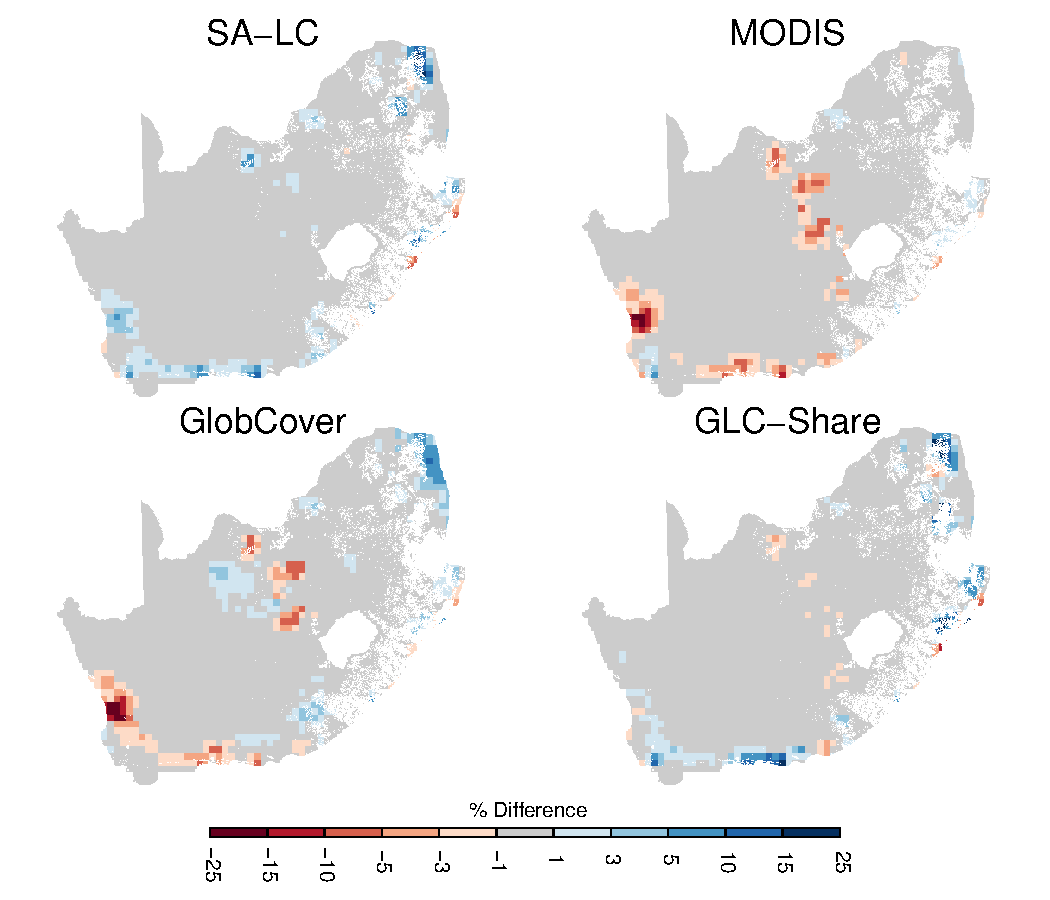
\includegraphics[width=.5\textwidth]{figures/et_bias_map.pdf}}
\caption{Differences in evapotranpiration estimates from a 29 year run of the VIC land surface hydrology model when initialized with LAI response curves derived from the reference map, versus those from the four cropland maps. Columns indicate differences between ET estimates from different portions of the model's time series: annual mean ET; highest annual ET value in the time series (TS max); smallest annual ET value in the time series (TS min); total of mean monthly ET for the three months having the highest ET during the year (Peak 3); the mean monthly ET of the peak ET month.}\label{afoto}
\end{figure}

\subsection{Initialization errors in spatial agent-based models}

\begin{itemize}
  \item We selected four magisterial districts with similar climates, and differing abundances of cropland ranging from X-Y\%, and differing patterns of map bias (Fig. S8). 
  \item Using household survey statistics from a project in Zambia that provides information on the average field area of farming households (X ha, SD = Y ha), we assigned each district a number of households determined by the total area of reference cropland in each district divided by mean farm size. \textcolor{red}{\textbf{Tom, Peng}, please correct as needed--maybe there is some variability to account for agent heterogeneity drawn by resampling from the distribution?}. This number of households represents the ``true'' number of households in the district.
  \item Disaggregated cropland to 100 m resolution, which is required by the model. 
  \item An agent-based model was then initialized wherein the household locations were seeded throughout the district, and assigned the required amount of cropland with a radius of X from the household location.
  \item These steps were repeated for each cropland map using the same number of household agents. 
  \item We then examined the differences that occurred between the agent initialization from the reference map and each of the four cropland maps, in terms of the percent of households that did not have cropland allocated, and the amount of cropland left unallocated in each district (Fig. 6).  
  \item The percent households without farms is 0 when cropland is overestimated (because there is plenty of land to choose from), but increases in a 1:1 relationship with the amount of cropland underestimation (positive values on X-axis in Fig. 6). \end{itemize} 

\vspace{-0.5 cm}
\begin{figure}[ht]
\centerline{\includegraphics[width=.3\textwidth]{figures/agent-bias.pdf}}
\caption{Biases in agent-based model initialization relative to cropland map biases, measured in terms of the percent of households having no cropland allocated (top) and the percent of cropland left unallocated (bottom). Dot sizes represent a district number (smallest = district 1; largest = district 4), colors represent the landcover map.  \textcolor{red}{to fix: add x-axis legend, add district number to legend.}}
\label{afoto}
\end{figure}

\begin{itemize}
  \item The percent of land unallocated, however, shows a U-shaped relationship with cropland biases, declining to near zero when cropland bias is between zero and up to $\sim$50\% under-estimated, thereafter increasing. Thus in cases where cropland bias insufficient farmland for households, a signficant share of available cropland can go unallocated (nearly 15\%).  \textcolor{red}{\textbf{Tom, Peng}, I assume this has to do something with seeding and the spatial pattern of cropland, but not sure exactly what. Model not sure which HH to give the land too because there are too many for the amount of cropland available, so it gives up? }
\end{itemize}

%large gradient ($\sim \displaystyle{ \inlinefrac{1}{\delta}}$).

\section{Discussion}

Some points to make thrown out now because out of time. Others will be added. Please add any important implications/considerations you see from the results.  

Some points from my notes last year: 
\begin{itemize}
  \item Bias as a function of scale
    \begin{enumerate}
      \item At 1 km resolution all landcover products are still fairly biased.  
       \item Bias drops to acceptable levels quickly for geowiki--at 5X5 km, mean bias is just 1\% (overestimated). The absolute bias for this dataset is 10\% or lower from 10X10 km resolution and coarser.  
       \item The SA dataset's bias is fairly consistent but low across all levels of aggregation, amounting to no more than an 8\% overestimate of cropland with absolute bias of similar magnitude. 
       \item MODIS and GlobCover biases (mostly of underestimation) do not dissipate until the higher levels of aggregation. MODIS's actual bias (under-estimation) falls below 10\% at 20 km resolution, but the absolute bias remains above 10\% until more than a 100-fold aggregation is done ($>$100 km resolution).  For GlobCover, it is still too high.  
    \end{enumerate}
  \item Bias as a function of cropland cover
    \begin{enumerate}
      \item Classification algorithms are thus more error-prone where landcover is mixed/heterogenous.
      \item The exception to this lies in the GlobCover dataset, where bias primarily increases as a function of cropland cover. The reason for this is that GlobCover's cropland classes do not provide for 100\% cropland cover, so aggregation tends to exacerbate underestimates. 
      \item Thus caution is needed when aggregating a mixed pixel class.  
        \begin{itemize} 
          \item An example illustrats this: take 4 1 km pixels, 2 of which are 100\% cropland, 2 of which are other cover types. Imagine a landcover product classifies 3 of these as cropland (2 correct, 1 an error of commission), using a cropland class that is defined as 50\% cropland. Aggregating the actual fraction by a factor of 4 will result in a new 4 km pixel having 50\% cropland, whereas aggregating the landcover product's pixels will give just 38\% cropland, even when factoring in the incorrect classification.)
          \end{itemize}
    \end{enumerate}
  \item Bias as a function of method
      \begin{enumerate}
        \item Higher resolution and ensemble-based approaches have less bias.
        \item geowiki represents a fusion of multiple coarse resolution data sources that has undergone extensive validation using a crowdsourcing approach
        \item the SALC dataset is based on 30 m landsat data, but incorporates a range of ancillary data and expert judgement
        \item MODIS and GlobCover data are effectively single source/single algorithm.
        \item \textbf{Newer points begin here}
        \item Statistically constrained constrained landcover estimation approaches provide accurate area-based inferences when aggregated. But spatial errors are still high, as seen with GeoWiki and production/yield estimates. Using these to identify yield gaps at specific map locations is inappropriate, or even for a larger location if it does not coincide with the geographic boundaries of the statistical unit.  
        \item Constrained estimates are also dependent on the accuracy of the statistics.  
    \end{enumerate}
  \item Fix above to have section on bias for global change studies
    \begin{enumerate}
      \item Scales at which it is safe to estimate values of say carbon stocks. 
      \item Above point about bias in disaggregated yield estimates - no point mapping these out. A new approach might be to take these statistically reported yields and then combine them with satellite data to estimate yield variability within the district.  That way would have meaningful reason for disaggregating yields, and would be pegged to real yield values, which would help minimize errors in remote sensing of yields. 
      \item Something on ET - doesn't seem to matter much, but land-atmosphere interactions can make these discrepancies meaningful, particularly since biases occur in arid areas where a lot of irrigation happens--can cause significant impacts on regional climate.  etc. etc. Also we didn't change out land cover types, and the vegetation in SA around the cropland will have reasonably similar LAI and ET responses (I think), thus impact more muted than it might be elsewhere (e.g. in forested landscapes).  
      \item Agent-based models. \textcolor{red}{Tom, Peng, something of significance/implications of this, please}
    \end{enumerate}
  \item Will need a section on way forward for data, etc. Key role of accurate landcover, particularly agricultural.  New methods, vectorized field boundaries seem to be highly valuable, Mapping Africa, Stephanie's paper, Geo-Wiki, etc are the way ahead.  
  
    
\end{itemize}




Mixed landscapes increase the chances of omission and commission errors by increasing the number of cover classes, or because such landscapes are less spectrally distinct \cite{estes_diylandcover:_2015}
% $\theta$ changes from 0 to 1. (see Figure \ref{afoto}).That means we are considering $\theta$  of the form
%For these solutions we have the following

%\begin{remark}
%Note that equation \eqref{theta} specifies  the function $\varphi$
%up to an error of order $\delta$. Theorem 1 provides an evolution
%equation for the function $\varphi$ up to an error of order
%$\delta |log \delta|$.
%\end{remark}

%(see \eqref{weaksol}). 
\subsection{More blather}


\begin{materials}
\section{Methods} 
Perhaps it is right {\it SI Materials and Methods}.

Describe weighted mean bias reasons. 

\section{Digital RCD Analysis} 

\end{materials}

\appendix[App 1]

\appendix
This is an example of an appendix without a title.

\begin{acknowledgments}
I thank everyone tearfully. 
\end{acknowledgments}


% bib solution from here
% http://tex.stackexchange.com/questions/167650/is-there-a-more-recent-bibliography-style-file-bst-for-pnas
% https://github.com/jburon/pnas2011.bst
\bibliographystyle{pnas2011} 
\bibliography{bias}

%\begin{thebibliography}{10}
%\bibitem{BN}
%M.~Belkin and P.~Niyogi, {\em Using manifold structure for partially
%  labelled classification}, Advances in NIPS, 15 (2003).
%
%\bibitem{BBG:EmbeddingRiemannianManifoldHeatKernel}
%P.~B\'erard, G.~Besson, and S.~Gallot, {\em Embedding {R}iemannian
%  manifolds by their heat kernel}, Geom. and Fun. Anal., 4 (1994),
%  pp.~374--398.
%\end{thebibliography}


\end{article}

%\begin{figure}
%\centerline{\includegraphics[width=.4\textwidth]{figsamp.eps}}
%\caption{LKB1 phosphorylates Thr-172 of AMPK$\alpha$ \textit{in vitro}
%and activates its kinase activity.}\label{afoto}
%\end{figure}
%
%\begin{figure*}[ht]
%\begin{center}
%\centerline{\includegraphics[width=.7\textwidth]{figsamp.eps}}
%\caption{LKB1 phosphorylates Thr-172 of AMPK$\alpha$ \textit{in vitro}
%and activates its kinase activity.}\label{afoto2}
%\end{center}
%\end{figure*}
%
%\begin{table}[h]
%\caption{Repeat length of longer allele by age of onset class.
%This is what happens when the text continues.}
%\begin{tabular}{@{\vrule height 10.5pt depth4pt  width0pt}lrcccc}
%&\multicolumn5c{Repeat length}\\
%\noalign{\vskip-11pt}
%Age of onset,\\
%\cline{2-6}
%\vrule depth 6pt width 0pt years&\multicolumn1c{\it n}&Mean&SD&Range&Median\\
%\hline
%Juvenile, 2$-$20&40&60.15& 9.32&43$-$86&60\\
%Typical, 21$-$50&377&45.72&2.97&40$-$58&45\\
%Late, $>$50&26&41.85&1.56&40$-$45&42\tablenote{The no. of wells for all samples was 384. Genotypes were
%determined by mass spectrometric assay. The $m_t$ value indicates the
%average number of wells positive for the over represented allele.}
%\\
%\hline
%\end{tabular}
%\end{table}
%
%
%\begin{table*}[ht]
%\caption{Summary of the experimental results}
%\begin{tabular*}{\hsize}
%{@{\extracolsep{\fill}}rrrrrrrrrrrrr}
%\multicolumn{3}{l}{Parameters}&
%\multicolumn{5}{c}{Averaged Results}&
%\multicolumn{5}{c}{Comparisons}\cr
%\hline
%\multicolumn1c{$n$}&\multicolumn1c{$S^*_{MAX}$}&
%\multicolumn1c{$t_1$}&\multicolumn1c{\ $r_1$}&
%\multicolumn1c{\ $m_1$}&\multicolumn1c{$t_2$}&
%\multicolumn1c{$r_2$}&\multicolumn1c{$m_2$}
%&\multicolumn1c{$t_{lb}$}&\multicolumn1c{\ \ $t_1/t_2$}&
%$r_1/r_2$&$m_1/m_2$&
%$t_1/t_{lb}$\cr
%\hline
%10\tablenote{Stanford Synchrotron Radiation Laboratory (Stanford University,
%Stanford, CA)}&1\quad &4&.0007&4&4&.0020&4&4&1.000&.333&1.000&1.000\cr
%10\tablenote{$R_{\rm FREE}=R$ factor for the $\sim 5$\% of the randomly
%chosen unique ref\/lections not used in the ref\/inement.}&5\quad &50&.0008&8&50&.0020&12&49&.999&.417&.698&1.020\cr
%100\tablenote{Calculated for all observed data}&20\quad &2840975&.0423&95&2871117&.1083&521&---&
%.990&.390&.182&---\ \ \cr
%\hline
%\end{tabular*}
%\end{table*}


\end{document}


